\newpage
\section{Auswertung}
\label{sec:auswertung}
\subsection{B-Feld Messung}
Da der Zeemann Effekt abhängig vom angelegten B-Feld ist un in diesem Versuchsaufbau nur der Spulenstrom zur Magnetfelderzeugung eingestellt werden kann muss zunächst der Zusammenhang zwischen Spulenstrom und Magnetfeld betrachtet werden.
Mit den Werten die wie in Abschnitt \ref{sec:BFeld} aufgenommen wurden wird ein linearer Fit und ein Fit eines Polynoms dritter Ordnung durchgeführt.
\begin{figure}[ht]
    \center
    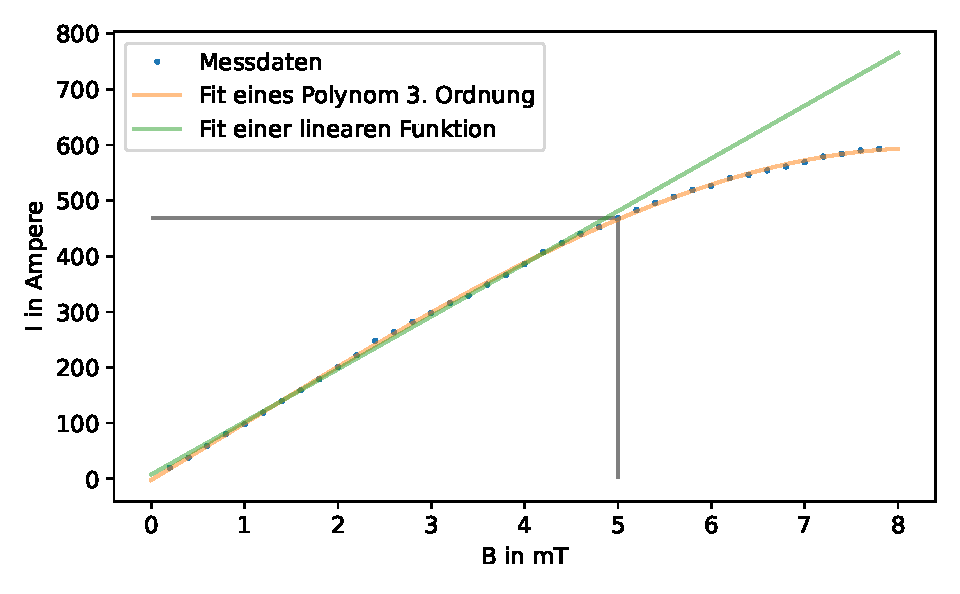
\includegraphics[width=0.65\textwidth]{plots/B_Feld.pdf}
    \caption{The rubidium fluorescence which is seen when the diode laser reaches the necessary energy to excite the rubidium gas. \cite{anleitungHeNe}}
    \label{fig:B_Feld}
\end{figure}
